\chapter{Phân tích và thiết kế hệ thống}
\label{ch:thiet-ke}

Chương này trình bày hệ thống Evidence Atlas: hệ thống phải làm được gì, được tổ chức ra sao, một câu hỏi đi qua những bước nào, và hệ thống làm gì để câu trả lời có căn cứ. Nội dung dựa trên tài liệu kiến trúc và tài liệu giao tiếp của dự án \src{14}, \src{23}.

\section{Yêu cầu của hệ thống}

\subsection{Người dùng và vai trò}

Hệ thống phục vụ hai vai trò:

\begin{itemize}
    \item \textbf{Người mua.} Hỏi để tìm sách, so sánh sách, xem người mua trước nói gì, hỏi về tác giả và nội dung tác phẩm. Người mua chỉ có quyền đọc dữ liệu.
    \item \textbf{Người bán.} Ngoài các việc trên, người bán xem được số liệu tổng hợp theo thể loại, tác giả, nhà xuất bản, mức giá, và được thử các thao tác quản lý trong một môi trường giả lập.
\end{itemize}

Người dùng chỉ chọn vai trò khi bắt đầu hội thoại. Danh tính, cửa hàng và phiên bản dữ liệu được dùng đều do máy chủ quyết định dựa trên khoá truy cập, không lấy từ nội dung người dùng gửi lên.

\subsection{Yêu cầu chức năng}

Bảng~\ref{tab:yc-chuc-nang} liệt kê mười chức năng chính mà hệ thống phải làm được.

\begin{table}[!htbp]
\caption{Các yêu cầu chức năng chính}
\label{tab:yc-chuc-nang}
\cobang
\begin{tabularx}{\linewidth}{C{1.1cm}P{4.2cm}Y}
\toprule
\textbf{STT} & \textbf{Chức năng} & \textbf{Mô tả}\\
\midrule
1 & Tìm và lọc sách & Tìm theo tên, tác giả, thể loại; lọc theo giá, điểm đánh giá, số trang.\\
2 & So sánh và xếp hạng & So sánh tối đa 5 cuốn theo điểm đánh giá, mức phổ biến và giá.\\
3 & Tóm tắt nhận xét & Tóm tắt điểm khen, điểm chê của người mua dựa trên các nhận xét được lấy mẫu.\\
4 & Đánh giá độ tin cậy & Nêu các dấu hiệu cần lưu ý trong nhận xét (lời phàn nàn, nhận xét quá ngắn hoặc lặp lại).\\
5 & Thống kê thị trường & Số liệu tổng hợp theo thể loại, tác giả, nhà xuất bản, khoảng giá.\\
6 & Hỏi về tác phẩm & Trả lời về tác giả, chủ đề, tên gốc của tác phẩm dựa trên kho tri thức, kèm trích dẫn.\\
7 & Hội thoại nhiều lượt & Nhớ các điều kiện và các cuốn sách đã nhắc ở lượt trước.\\
8 & Đề xuất thao tác & Chuẩn bị các thao tác như thêm vào giỏ, tạo đơn trong môi trường giả lập; chỉ thực hiện sau khi người dùng xác nhận.\\
9 & Theo dõi tiến trình & Hiển thị các bước hệ thống đang làm và cho phép huỷ giữa chừng.\\
10 & Từ chối có lý do & Khi không đủ căn cứ, nói rõ thiếu gì hoặc hỏi lại, không đoán.\\
\bottomrule
\end{tabularx}
\end{table}

\subsection{Yêu cầu phi chức năng}

\begin{itemize}
    \item \textbf{Có căn cứ.} Mỗi nhận định về tác phẩm phải chỉ được tới một đoạn nguồn cụ thể. Số liệu về giá, điểm đánh giá, số trang phải lấy nguyên từ danh mục, không để mô hình tự viết ra.
    \item \textbf{Có giới hạn.} Mỗi lượt hỏi có hạn mức rõ ràng về số bước, số lần tra cứu, thời gian chờ và chi phí.
    \item \textbf{An toàn.} Mọi yêu cầu đều phải xác thực. Quyền được kiểm tra ở máy chủ, không dựa vào việc ẩn nút trên giao diện. Thông báo lỗi không để lộ nội dung nội bộ.
    \item \textbf{Bền vững.} Hội thoại, lượt hỏi và kết quả được lưu trong cơ sở dữ liệu. Mất kết nối hoặc gửi lại yêu cầu không làm mất dữ liệu và không tạo bản ghi trùng.
    \item \textbf{Lặp lại được.} Dữ liệu, kho tri thức và cấu hình mô hình đều có phiên bản. Có thể chạy lại một thực nghiệm với đúng các thành phần đã dùng.
    \item \textbf{Dễ dùng.} Giao diện và thông báo bằng tiếng Việt; dùng được bằng bàn phím; hiển thị rõ các trạng thái đang tải, thành công một phần, lỗi và mất mạng.
\end{itemize}

\subsection{Những việc hệ thống không làm}

Để tránh hiểu lầm, nhóm nêu rõ các việc nằm ngoài phạm vi:

\begin{itemize}
    \item không thực hiện giao dịch thật; mọi thao tác mua bán chỉ diễn ra trong môi trường giả lập;
    \item không khẳng định một nhận xét là giả hay một người bán là gian lận, chỉ nêu dấu hiệu;
    \item không đưa ra nhận định về xu hướng theo thời gian hay tình hình hiện tại, vì dữ liệu là một bản chụp trong quá khứ và không có mốc thời gian;
    \item không cam kết loại bỏ hoàn toàn thông tin sai; bước kiểm chứng tự động có sai số.
\end{itemize}

\section{Nguyên tắc thiết kế}

Bốn nguyên tắc sau chi phối các quyết định thiết kế trong chương.

\textbf{Thứ nhất, chương trình quyết định, mô hình đề xuất.} Mô hình ngôn ngữ giỏi hiểu câu hỏi và viết câu trả lời, nhưng có thể sai mà không báo trước. Vì vậy mọi việc liên quan đến quyền, hạn mức, số liệu và việc gắn nguồn đều do chương trình thông thường đảm nhiệm. Mô hình chỉ được chọn trong những phương án mà chương trình cho phép.

\textbf{Thứ hai, bằng chứng trước, trình bày sau.} Câu trả lời được xây từ các dữ kiện và đoạn nguồn đã thu thập, không phải từ trí nhớ của mô hình. Không có bằng chứng thì không có nhận định.

\textbf{Thứ ba, giới hạn rõ ràng.} Số chuyên gia là cố định. Số bước của một lượt hỏi có trần. Hệ thống không cho các tác tử tự do trao đổi qua lại, vì cách đó khó kiểm soát chi phí và khó tìm nguyên nhân khi sai.

\textbf{Thứ tư, trung thực khi gặp sự cố.} Khi một phần việc thất bại, hệ thống nói rõ phần nào làm được, phần nào không, thay vì im lặng trả về một câu trả lời trông như đầy đủ.

\section{Kiến trúc tổng thể}

Hệ thống được xây dựng dưới dạng một ứng dụng duy nhất chia thành các khối chức năng, chạy trong một tiến trình. Nhóm không tách thành nhiều dịch vụ nhỏ, vì quy mô đề tài không cần đến và cách này đơn giản hơn khi triển khai, kiểm thử. Hình~\ref{fig:kien-truc} cho thấy các tầng của hệ thống.

\hinh{kien-truc}{Kiến trúc tổng thể của Evidence Atlas}{fig:kien-truc}

\textbf{Giao diện web.} Trang web nơi người dùng trò chuyện với trợ lý. Giao diện được chính máy chủ của hệ thống phục vụ, nên không cần cấu hình riêng cho việc gọi chéo giữa hai địa chỉ.

\textbf{Cổng tiếp nhận.} Mọi yêu cầu đều đi qua đây. Cổng xác thực khoá truy cập, xác định người dùng là ai và có quyền gì, giới hạn số yêu cầu của mỗi người dùng trong một khoảng thời gian, và gắn cho mỗi yêu cầu một mã theo dõi để tra cứu khi có sự cố.

\textbf{Lõi điều phối.} Phần trung tâm, gồm ba việc: lập kế hoạch trong giới hạn cho phép, thực thi lần lượt các bước, và soạn rồi kiểm chứng câu trả lời.

\textbf{Bốn chuyên gia cố định.} Mỗi chuyên gia phụ trách một loại việc và chỉ được dùng các công cụ thuộc phạm vi của mình (Mục~\ref{sec:chuyen-gia}).

\textbf{Cơ sở dữ liệu.} Một cơ sở dữ liệu PostgreSQL lưu tất cả: danh mục sách và nhận xét, kho tri thức, các hội thoại, lượt hỏi, và sổ ghi chi phí. Các chuyên gia chỉ được \emph{đọc} dữ liệu, và mọi lần đọc đều đi qua một cổng công cụ có kiểm tra quyền.

\textbf{Mô hình ngôn ngữ.} Là dịch vụ bên ngoài. Hệ thống gửi yêu cầu tới mô hình ở một số bước nhất định và luôn yêu cầu mô hình trả lời theo một khuôn mẫu có cấu trúc để chương trình kiểm tra được.

\section{Một câu hỏi được xử lý như thế nào}
\label{sec:vong-doi}

Hình~\ref{fig:vong-doi} mô tả chín bước mà một lượt hỏi đi qua. Các ô trắng là bước do chương trình quyết định hoàn toàn; các ô xám là bước có mô hình ngôn ngữ tham gia.

\hinh{vong-doi-luot-hoi}{Chín bước xử lý một lượt hỏi}{fig:vong-doi}

\textbf{Bước 1 -- Tiếp nhận.} Hệ thống xác thực người gửi, kiểm tra quyền và ghi lượt hỏi vào cơ sở dữ liệu trước khi làm bất cứ việc gì khác. Một yêu cầu chỉ gồm ba thông tin: hội thoại nào, mã lượt hỏi do phía người dùng tạo ra, và nội dung câu hỏi (tối đa 2.000 ký tự).

\textbf{Bước 2 -- Ghim phiên bản.} Hệ thống ghi lại phiên bản danh mục và phiên bản kho tri thức sẽ dùng cho lượt hỏi này. Nếu chưa có kho tri thức nào được công bố, hoặc mô hình tìm kiếm không khớp với kho, hệ thống từ chối phục vụ thay vì chạy với dữ liệu không chắc chắn.

\textbf{Bước 3 -- Hiểu câu hỏi.} Chương trình nhận ra các thông tin cụ thể trong câu hỏi: tên sách, mức giá, điểm đánh giá tối thiểu, số trang. Việc này dùng quy tắc, không dùng mô hình, để các con số trong câu hỏi không bị diễn giải sai.

\textbf{Bước 4 -- Lập kế hoạch.} Mô hình đọc câu hỏi và đề xuất danh sách các bước cần làm, mỗi bước là một việc giao cho một chuyên gia. Mô hình chỉ được chọn trong danh sách các việc mà chương trình cho phép.

\textbf{Bước 5 -- Duyệt kế hoạch.} Chương trình kiểm tra kế hoạch: người dùng có quyền làm từng việc không, các bước có đúng thứ tự phụ thuộc không, tổng số bước có vượt hạn mức không. Kế hoạch không hợp lệ thì bị từ chối.

\textbf{Bước 6 -- Thực thi.} Các bước được chạy lần lượt. Mỗi chuyên gia trả về hai loại kết quả: \emph{dữ kiện} (ví dụ giá của một cuốn sách) và \emph{bằng chứng} (ví dụ một đoạn trong kho tri thức).

\textbf{Bước 7 -- Soạn câu trả lời.} Mô hình nhận danh sách dữ kiện và bằng chứng, chọn những phần liên quan, rồi viết phần diễn giải. Các con số từ danh mục được chương trình chèn vào nguyên văn; mô hình không được viết lại.

\textbf{Bước 8 -- Kiểm chứng.} Từng nhận định trong bản nháp được đối chiếu với đoạn nguồn (Mục~\ref{sec:kiem-chung}).

\textbf{Bước 9 -- Trả kết quả.} Người dùng nhận được một trong ba loại phản hồi: câu trả lời kèm nguồn; một câu hỏi lại để làm rõ; hoặc lời từ chối có nêu lý do.

Trong lúc chờ, giao diện nhận được các thông báo tiến trình (đang làm bước nào) và từng phần của câu trả lời ngay khi có. Mỗi lượt hỏi kết thúc bằng đúng một thông báo cuối cùng. Nếu kết nối bị ngắt giữa chừng, giao diện có thể hỏi lại máy chủ để lấy trạng thái và kết quả của lượt hỏi đó.

\section{Bốn chuyên gia}
\label{sec:chuyen-gia}

\subsection{Phân công}

Hệ thống có đúng bốn chuyên gia, không thêm bớt lúc chạy. Bảng~\ref{tab:chuyen-gia} nêu việc của từng chuyên gia và giới hạn tương ứng.

\begin{table}[!htbp]
\caption{Bốn chuyên gia: nhiệm vụ và giới hạn}
\label{tab:chuyen-gia}
\cobang
\begin{tabularx}{\linewidth}{P{2.4cm}YY}
\toprule
\textbf{Chuyên gia} & \textbf{Làm gì} & \textbf{Không làm gì}\\
\midrule
Sản phẩm & Tìm, lọc, so sánh và xếp hạng sách dựa trên thông tin trong danh mục. & Không nhận xét về nội dung tác phẩm.\\
Đánh giá & Lấy mẫu nhận xét của người mua; tóm tắt điểm khen, điểm chê theo từng khía cạnh; so sánh nhận xét giữa các cuốn. & Không coi mẫu nhận xét là đại diện cho mọi người mua.\\
Độ tin cậy & Nêu các dấu hiệu cần lưu ý: tỉ lệ phàn nàn, nhận xét quá ngắn hoặc lặp lại. & Không khẳng định nhận xét giả, hàng giả hay gian lận.\\
Thị trường & Tính số liệu tổng hợp theo thể loại, tác giả, nhà xuất bản, khoảng giá, mức điểm. & Không nói về xu hướng theo thời gian hay tình hình hiện tại.\\
\bottomrule
\end{tabularx}
\end{table}

Việc tra cứu kho tri thức không thuộc riêng chuyên gia nào. Đó là một năng lực dùng chung, được gọi khi câu hỏi liên quan đến bản thân tác phẩm.

\subsection{Cách phối hợp}

Hình~\ref{fig:phoi-hop} cho thấy cách các thành phần làm việc với nhau.

\hinh{phoi-hop-chuyen-gia}{Bộ điều phối giao việc cho bốn chuyên gia và gom kết quả}{fig:phoi-hop}

Cách phối hợp này có ba đặc điểm, khác với nhiều hệ nhiều tác tử được mô tả trong tài liệu:

\begin{itemize}
    \item \textbf{Các chuyên gia không nói chuyện với nhau.} Chuyên gia chỉ nhận việc từ bộ điều phối và trả kết quả về. Không có thương lượng hay tranh luận giữa các chuyên gia.
    \item \textbf{Các chuyên gia không có bộ nhớ riêng.} Mọi thông tin cần nhớ nằm ở bộ điều phối và cơ sở dữ liệu.
    \item \textbf{Các bước chạy lần lượt.} Bước sau có thể dùng kết quả của bước trước. Ví dụ với câu hỏi so sánh, chuyên gia sản phẩm chọn ra tối đa 5 cuốn trước; chuyên gia đánh giá so sánh nhận xét của đúng các cuốn đó; rồi chuyên gia độ tin cậy xem xét nhận xét của chúng.
\end{itemize}

Khi một bước thất bại, cách xử lý tuỳ vào vai trò của bước đó. Nếu chuyên gia sản phẩm không tìm được cuốn nào, các bước sau không có gì để làm và hệ thống báo là không tìm thấy. Nếu một bước phụ thất bại (ví dụ không lấy được nhận xét), hệ thống vẫn trả lời phần đã có và kèm cảnh báo về phần thiếu.

\subsection{Công thức xếp hạng}

Khi người dùng nhờ gợi ý, chuyên gia sản phẩm xếp hạng các cuốn sách bằng một công thức cố định, không để mô hình tự chọn theo cảm tính:

\[
\text{Điểm xếp hạng} = 0{,}45 \times \frac{r}{5} \;+\; 0{,}35 \times \frac{\log(1+p)}{\log(1+p_{\max})} \;+\; 0{,}20 \times \left(1 - \frac{g}{g_{\max}}\right)
\]

Trong đó $r$ là điểm đánh giá trung bình (thang 5), $p$ là mức phổ biến, $g$ là giá bán; $p_{\max}$ và $g_{\max}$ là giá trị lớn nhất trong nhóm sách đang xét. Điểm đánh giá có trọng số lớn nhất (45\%), tiếp đến là mức phổ biến (35\%) và giá (20\%, giá càng thấp điểm càng cao). Mức phổ biến được lấy lô-ga-rít để một vài cuốn bán rất chạy không lấn át toàn bộ kết quả.

Dùng công thức cố định có hai lợi ích: cùng một câu hỏi luôn cho cùng một thứ tự, và hệ thống giải thích được vì sao cuốn này xếp trên cuốn kia. Như đã nêu ở Chương~\ref{ch:du-lieu}, mức phổ biến là con số do nguồn cung cấp, chưa được kiểm chứng là doanh số thật.

\section{Lập kế hoạch có giới hạn}

\subsection{Phân chia việc giữa chương trình và mô hình}

Bảng~\ref{tab:phan-chia} tóm tắt ai làm việc gì. Đây là quyết định thiết kế quan trọng nhất của hệ thống.

\begin{table}[!htbp]
\caption{Phân chia việc giữa chương trình và mô hình ngôn ngữ}
\label{tab:phan-chia}
\cobang
\begin{tabularx}{\linewidth}{YY}
\toprule
\textbf{Chương trình quyết định} & \textbf{Mô hình được làm}\\
\midrule
Nhận ra tên sách, giá, điểm đánh giá trong câu hỏi & Đề xuất các bước cần làm, chọn từ danh sách cho phép\\
Người dùng có quyền làm việc gì & Chọn dữ kiện và bằng chứng nào liên quan đến câu hỏi\\
Thứ tự phụ thuộc giữa các bước & Viết phần diễn giải bằng lời tự nhiên\\
Nội dung các dữ kiện từ danh mục (giá, điểm, số trang) & Sửa bản nháp một lần khi bị bước kiểm chứng trả lại\\
Điểm xếp hạng và trạng thái của từng bước & \\
Gắn nhận định với đoạn nguồn và đánh số trích dẫn & \\
\bottomrule
\end{tabularx}
\end{table}

\subsection{Các hạn mức}

Mỗi lượt hỏi chịu các hạn mức ở Bảng~\ref{tab:han-muc}. Hạn mức giúp chi phí và thời gian của một lượt hỏi luôn có trần, kể cả khi mô hình đề xuất một kế hoạch quá dài.

\begin{table}[!htbp]
\caption{Các hạn mức áp dụng cho một lượt hỏi}
\label{tab:han-muc}
\cobang
\begin{tabularx}{\linewidth}{YR{4.2cm}}
\toprule
\textbf{Hạn mức} & \textbf{Giá trị}\\
\midrule
Độ dài câu hỏi & tối đa 2.000 ký tự\\
Số bước giao cho chuyên gia & tối đa 8\\
Số lần chỉnh kế hoạch & tối đa 1\\
Số bước đọc được thêm khi chỉnh kế hoạch & tối đa 2\\
Số sách đưa vào so sánh, xếp hạng & tối đa 5\\
Số lần tra cứu kho tri thức & tối đa 2\\
Số câu truy vấn trong một lần tra cứu & tối đa 4\\
Lượng văn bản tra cứu đưa cho mô hình & tối đa 6.000 token\\
Số lần cho mô hình sửa bản nháp & tối đa 1\\
Số kết quả trung gian được giữ lại & tối đa 16\\
\bottomrule
\end{tabularx}
\end{table}

\subsection{Kế hoạch cố định và kế hoạch thích ứng}

Hệ thống hỗ trợ hai cách lập kế hoạch, và đây cũng là một yếu tố được so sánh trong thực nghiệm:

\begin{itemize}
    \item \textbf{Kế hoạch cố định.} Chương trình tự lập kế hoạch theo quy tắc định sẵn dựa trên loại câu hỏi, không hỏi mô hình. Kế hoạch được giữ nguyên đến khi xong.
    \item \textbf{Kế hoạch thích ứng.} Mô hình đề xuất kế hoạch. Sau khi có kết quả ban đầu, hệ thống được phép bổ sung kế hoạch đúng một lần, ví dụ thêm một bước tra cứu khi thấy còn thiếu thông tin.
\end{itemize}

Kế hoạch thích ứng linh hoạt hơn nhưng tốn thêm lượt gọi mô hình. Việc linh hoạt đó có đáng giá hay không là một câu hỏi được trả lời bằng số liệu ở Chương~\ref{ch:ket-qua}.

\section{Kiểm chứng câu trả lời}
\label{sec:kiem-chung}

Đây là cơ chế chống ảo giác chính của hệ thống. Hình~\ref{fig:kiem-chung} mô tả quy trình.

\hinh{kiem-chung}{Quy trình kiểm chứng từng nhận định trước khi trả lời}{fig:kiem-chung}

Bản nháp do mô hình viết không được gửi thẳng cho người dùng. Bản nháp được tách thành từng nhận định, và với mỗi nhận định, mô hình phải chỉ ra đoạn nguồn làm căn cứ. Sau đó có hai lần kiểm tra:

\begin{itemize}
    \item \textbf{Kiểm tra 1 -- đoạn nguồn có thật không.} Chương trình kiểm tra đoạn được trích có đúng là nằm trong tài liệu, đúng phiên bản đã ghim, đúng vị trí. Lần kiểm tra này là so khớp chính xác, không dùng mô hình, nên không thể bị ``thuyết phục''. Nó chặn trường hợp mô hình bịa ra một trích dẫn.
    \item \textbf{Kiểm tra 2 -- đoạn nguồn có nói điều đó không.} Một trích dẫn có thật vẫn có thể không liên quan đến nhận định. Lần kiểm tra này xét xem nội dung đoạn nguồn có thực sự dẫn tới nhận định hay không.
\end{itemize}

Nhận định đạt cả hai kiểm tra thì được giữ và gắn số trích dẫn. Nhận định không đạt được trả lại cho mô hình sửa, nhưng \emph{chỉ một lần}. Nếu vẫn không đạt, nhận định bị bỏ khỏi câu trả lời, hoặc hệ thống nói rõ là không đủ căn cứ.

Giới hạn sửa một lần là có chủ ý. Cho sửa nhiều lần làm tăng chi phí và tạo điều kiện để mô hình ``thử cho đến khi lọt''. Một lần sửa đủ để xử lý các lỗi diễn đạt, còn các nhận định thật sự không có căn cứ thì nên bị loại.

Cần nói rõ giới hạn của cơ chế này. Kiểm tra 2 là một phép kiểm tra tự động và có sai số; nó có thể bỏ lọt một nhận định sai hoặc loại nhầm một nhận định đúng. Nhóm vì vậy không khẳng định hệ thống loại bỏ hoàn toàn thông tin sai, mà chỉ khẳng định mỗi nhận định được giữ lại đều chỉ tới một đoạn nguồn có thật để người đọc tự kiểm tra.

\section{Lưu trạng thái và độ bền}

\subsection{Trạng thái của một lượt hỏi}

Mỗi lượt hỏi được lưu trong cơ sở dữ liệu cùng trạng thái của nó. Hình~\ref{fig:trang-thai} cho thấy các trạng thái có thể có.

\hinh{trang-thai-luot}{Các trạng thái của một lượt hỏi}{fig:trang-thai}

Một lượt hỏi bắt đầu ở trạng thái \emph{chờ xử lý}, chuyển sang \emph{đang chạy}, rồi kết thúc ở một trong bốn trạng thái: \emph{hoàn tất}, \emph{thất bại}, \emph{đã huỷ} (người dùng bấm huỷ) hoặc \emph{bị gián đoạn} (máy chủ dừng giữa chừng).

\subsection{Gửi lại không tạo bản ghi trùng}

Trên thực tế, mạng có thể chập chờn và giao diện có thể gửi lại một yêu cầu. Để việc gửi lại an toàn, mỗi lượt hỏi mang một mã do phía người dùng tạo. Khi máy chủ nhận một yêu cầu có mã đã gặp, máy chủ không chạy lại mà trả về trạng thái hoặc kết quả đã lưu. Nếu yêu cầu gửi lại không khớp với lượt hỏi đã lưu, máy chủ báo xung đột thay vì âm thầm ghi đè.

Cùng nguyên tắc này áp dụng cho việc xác nhận thao tác: yêu cầu xác nhận phải kèm một mã riêng, nên bấm xác nhận hai lần cũng chỉ thực hiện một lần.

\subsection{Chỉ một nơi xử lý một lượt hỏi}

Khi có nhiều tiến trình cùng phục vụ, cần bảo đảm một lượt hỏi không bị hai tiến trình xử lý song song. Hệ thống dùng chính cơ sở dữ liệu để làm việc này: tiến trình nào nhận xử lý thì ghi tên mình và thời hạn giữ vào bản ghi của lượt hỏi; tiến trình khác thấy bản ghi đang có chủ thì bỏ qua. Nếu một tiến trình bị treo quá thời hạn, tiến trình khác được nhận lại; kết quả gửi về muộn của tiến trình cũ sẽ bị từ chối.

\section{Bộ nhớ hội thoại}

Hệ thống có ba lớp bộ nhớ với mục đích khác nhau:

\begin{itemize}
    \item \textbf{Lịch sử hội thoại.} Toàn bộ câu hỏi và câu trả lời được lưu bền vững để người dùng xem lại.
    \item \textbf{Ngữ cảnh đưa cho mô hình.} Chỉ một phần lịch sử được đưa vào mỗi lượt hỏi: tối đa 8 lượt gần nhất đã hoàn tất, tối đa 16 điều kiện đã nêu (ví dụ ``dưới 150.000 đồng''), và tối đa 8 cuốn sách đã nhắc tới. Giới hạn này giữ cho chi phí mỗi lượt không tăng dần theo độ dài hội thoại.
    \item \textbf{Sở thích do người dùng tự khai.} Người dùng có thể lưu tối đa 4 mục sở thích. Hệ thống chỉ ghi nhớ những gì người dùng chủ động lưu, và người dùng xem, sửa, xoá được bất cứ lúc nào.
\end{itemize}

Hệ thống không tự suy ra sở thích từ nội dung trò chuyện. Lựa chọn này làm trợ lý kém ``thông minh'' hơn một chút nhưng người dùng luôn biết hệ thống đang nhớ gì về mình.

\section{An toàn và phân quyền}

\subsection{Xác thực và quyền}

Mỗi yêu cầu phải kèm một khoá truy cập. Máy chủ đối chiếu khoá với danh sách người dùng được cấu hình sẵn; từ đó biết người dùng thuộc cửa hàng nào và có những quyền gì. Người dùng không có trong danh sách bị từ chối. Trên trình duyệt, khoá chỉ được giữ trong bộ nhớ tạm của trang và mất khi đóng trang; khoá không được lưu xuống ổ đĩa của trình duyệt.

Quyền được kiểm tra ở ba tầng: ở cổng tiếp nhận (người này có được gọi chức năng này không), ở bước duyệt kế hoạch (kế hoạch có bước nào vượt quyền không), và ở cổng công cụ (lần đọc dữ liệu này có được phép không). Mỗi tài nguyên như hội thoại, lượt hỏi, đề xuất thao tác đều gắn với chủ sở hữu; người khác không đọc được.

\subsection{Thao tác cần xác nhận}

Trợ lý không tự thực hiện thao tác nào làm thay đổi dữ liệu. Với các yêu cầu như thêm vào giỏ hay tạo đơn, hệ thống chỉ chuẩn bị một \emph{đề xuất} và chờ. Người dùng xem nội dung đề xuất rồi chọn xác nhận hoặc từ chối. Nếu trong lúc soạn, mô hình thay đổi danh sách sách so với danh sách đã được chương trình duyệt, đề xuất bị loại.

Mọi thao tác kiểu này diễn ra trong môi trường giả lập. Không có đơn hàng thật, không có thanh toán thật.

\subsection{Giảm rủi ro khi dùng mô hình bên ngoài}

\begin{itemize}
    \item Nội dung do người dùng nhập và nội dung nhận xét được coi là dữ liệu, không phải mệnh lệnh. Một nhận xét có chứa câu kiểu ``hãy bỏ qua các hướng dẫn trước'' không làm thay đổi hành vi của hệ thống, vì quyền và kế hoạch do chương trình kiểm soát.
    \item Mô hình luôn phải trả lời theo khuôn mẫu có cấu trúc. Câu trả lời sai khuôn mẫu bị loại.
    \item Hệ thống yêu cầu nhà cung cấp mô hình không lưu lại nội dung các yêu cầu.
    \item Nhật ký theo dõi được rút gọn và che các phần nhạy cảm. Thông báo lỗi gửi cho người dùng không chứa nội dung hướng dẫn nội bộ, dữ liệu trung gian hay thông tin đăng nhập.
    \item Dữ liệu từ máy chủ được giao diện hiển thị dưới dạng văn bản thuần, không được chạy như mã lệnh.
\end{itemize}

\section{Kiểm soát chi phí và sự cố}

Gọi mô hình ngôn ngữ tốn tiền và có thể chậm hoặc lỗi. Hệ thống có các cơ chế sau:

\begin{itemize}
    \item \textbf{Sổ ghi chi phí.} Mỗi lượt gọi mô hình được ghi lại số token và chi phí ước tính vào cơ sở dữ liệu. Nhờ sổ này, mọi con số về chi phí trong Chương~\ref{ch:ket-qua} đều là số đo, không phải ước lượng.
    \item \textbf{Hạn mức ngân sách.} Khi tổng chi phí chạm trần đã đặt, hệ thống ngừng gọi mô hình.
    \item \textbf{Giới hạn thời gian chờ và số lần thử lại.} Mỗi lượt gọi có thời gian chờ tối đa; quá thời gian thì bị huỷ.
    \item \textbf{Ngắt mạch.} Khi dịch vụ mô hình lỗi liên tiếp, hệ thống tạm ngừng gọi trong một khoảng thời gian thay vì tiếp tục gửi yêu cầu chắc chắn thất bại.
    \item \textbf{Chế độ dùng mô hình.} Người vận hành chọn được một trong bốn chế độ: tắt mô hình (chỉ dùng quy tắc), chạy thử song song (mô hình chạy nhưng kết quả không được dùng), kết hợp (dùng mô hình, lỗi thì quay về quy tắc), và bắt buộc (lỗi mô hình thì báo lỗi).
\end{itemize}

\section{Giao tiếp với hệ thống}

Giao diện web và các chương trình khác làm việc với hệ thống qua một bộ chức năng được liệt kê ở Bảng~\ref{tab:giao-tiep}.

\begin{table}[!htbp]
\caption{Các nhóm chức năng hệ thống cung cấp cho bên ngoài}
\label{tab:giao-tiep}
\cobang
\begin{tabularx}{\linewidth}{P{3.4cm}Y}
\toprule
\textbf{Nhóm} & \textbf{Chức năng}\\
\midrule
Danh tính & Cho biết người dùng hiện tại là ai và được dùng những vai trò nào.\\
Hội thoại & Tạo hội thoại mới; liệt kê các hội thoại của mình; đọc lại một hội thoại; xoá hội thoại.\\
Hỏi đáp & Gửi câu hỏi và nhận câu trả lời một lần; hoặc gửi câu hỏi và nhận tiến trình cùng câu trả lời từng phần.\\
Lượt hỏi & Đọc trạng thái và kết quả của một lượt hỏi; huỷ một lượt hỏi đang chạy.\\
Đề xuất thao tác & Đọc nội dung một đề xuất; xác nhận; từ chối.\\
Sở thích & Đọc, lưu và xoá các sở thích tự khai.\\
Vận hành & Kiểm tra hệ thống còn sống và đã sẵn sàng chưa; xem số liệu vận hành. Các chức năng xem nhật ký chi tiết cần một khoá riêng dành cho người vận hành.\\
\bottomrule
\end{tabularx}
\end{table}

Mỗi phản hồi đều kèm mã theo dõi của yêu cầu. Khi người dùng báo lỗi, chỉ cần mã này là người vận hành tìm được toàn bộ quá trình xử lý tương ứng.

\section{Giao diện người dùng}

Giao diện là một trang web gồm ba vùng (Hình~\ref{fig:giao-dien}):

\begin{itemize}
    \item \textbf{Vùng trái -- các tác tử.} Liệt kê bộ điều phối và các chuyên gia tham gia lượt hỏi hiện tại, kèm trạng thái của từng thành phần.
    \item \textbf{Vùng giữa -- hội thoại.} Nơi người dùng chọn vai trò, nhập câu hỏi và đọc câu trả lời. Mỗi nhận định có số trích dẫn đặt ngay bên cạnh. Các đề xuất thao tác hiện thành thẻ riêng với nút xem và xác nhận.
    \item \textbf{Vùng phải -- chi tiết thực thi.} Hiển thị kế hoạch đã chạy, mức sử dụng, danh sách nguồn bằng chứng tương ứng với các số trích dẫn, và các mã theo dõi.
\end{itemize}

Cách bố trí này phục vụ nguyên tắc ``bằng chứng trước'': người dùng không chỉ thấy câu trả lời mà còn thấy câu trả lời đến từ đâu và hệ thống đã làm những bước nào. Giao diện tự xếp lại thành một cột trên điện thoại.

\begin{figure}[p]
    \centering
    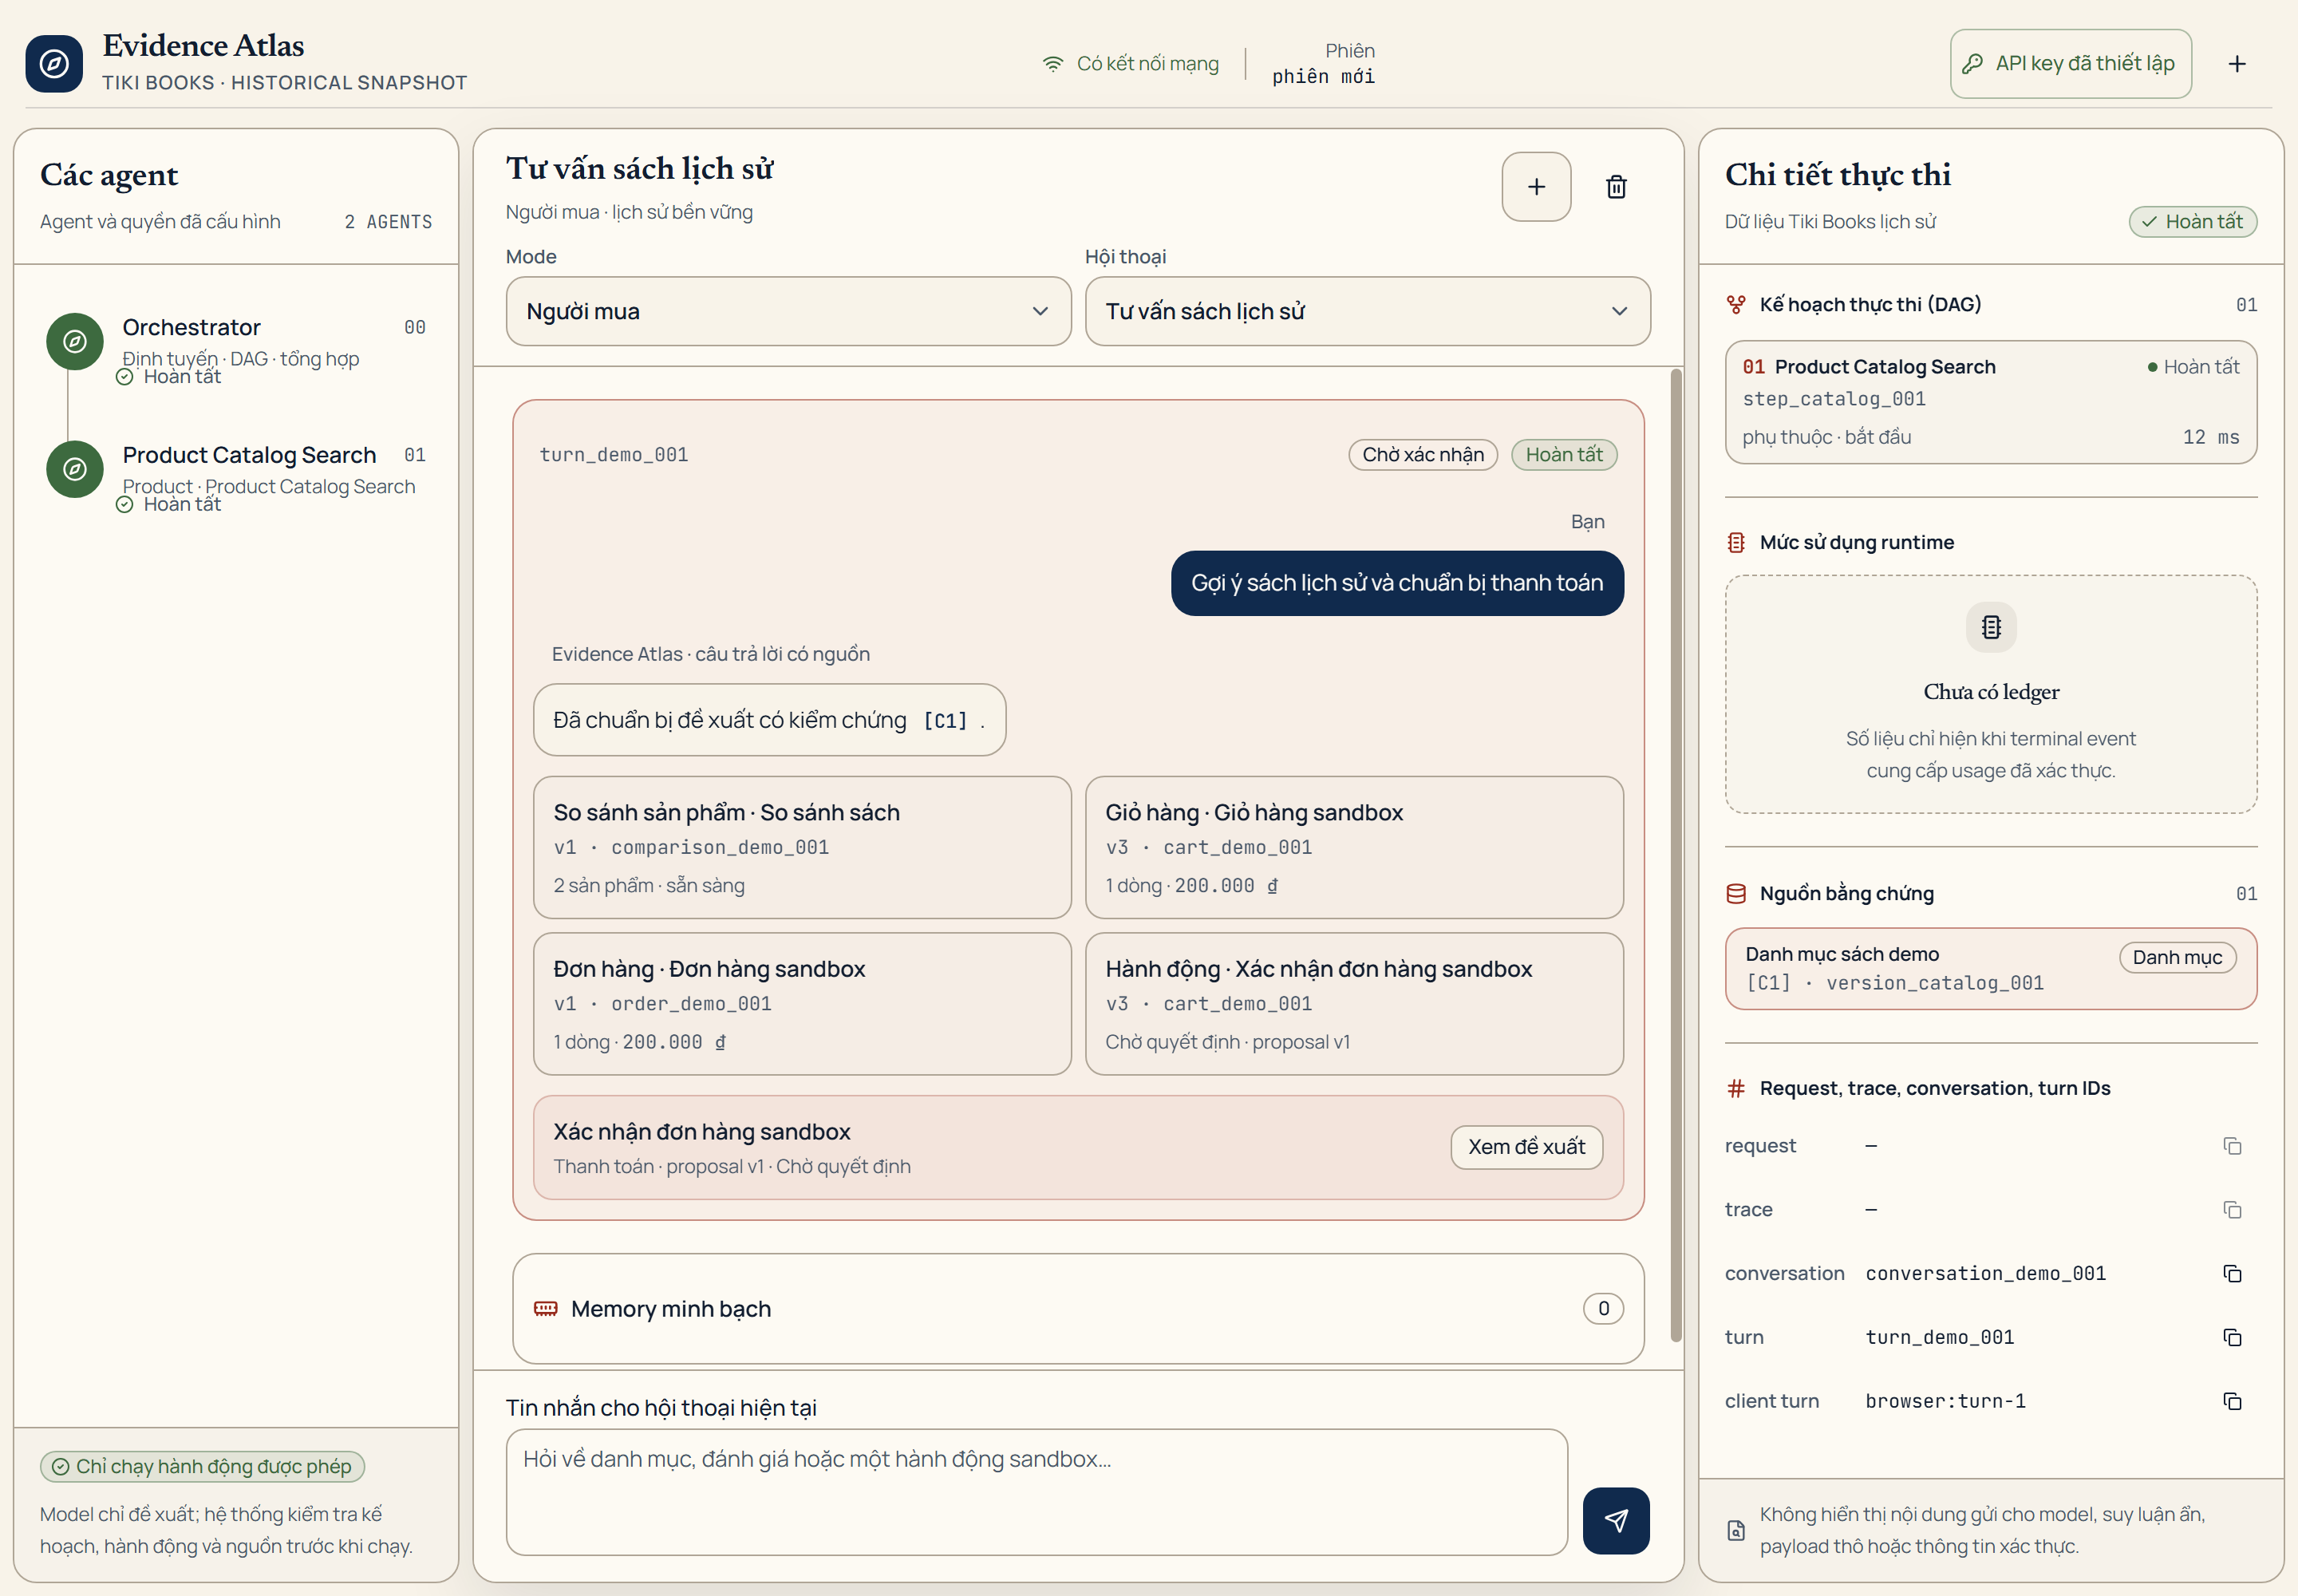
\includegraphics[angle=90,width=0.93\linewidth]{images/giao-dien.png}
    \caption{Giao diện Evidence Atlas (ảnh xoay ngang; chụp với dữ liệu minh hoạ của bản kiểm thử giao diện, không phải kết quả thực nghiệm)}
    \label{fig:giao-dien}
\end{figure}

\section{Công nghệ sử dụng}

Bảng~\ref{tab:cong-nghe} liệt kê các công nghệ chính và lý do chọn từng công nghệ.

\begin{table}[!htbp]
\caption{Các công nghệ chính}
\label{tab:cong-nghe}
\cobang
\begin{tabularx}{\linewidth}{P{3.6cm}P{4.6cm}Y}
\toprule
\textbf{Thành phần} & \textbf{Công nghệ} & \textbf{Lý do chọn}\\
\midrule
Máy chủ & Python, FastAPI & Hỗ trợ tốt xử lý bất đồng bộ và trả kết quả từng phần.\\
Cơ sở dữ liệu & PostgreSQL & Lưu được cả dữ liệu thông thường lẫn véc-tơ tìm kiếm trong một nơi; hỗ trợ giao dịch.\\
Giao diện & React, TypeScript, Vite & Phổ biến, có kiểm tra kiểu giúp giảm lỗi.\\
Kiểu dáng giao diện & Tailwind CSS, shadcn/ui & Bộ thành phần có sẵn, hỗ trợ bàn phím và trình đọc màn hình.\\
Mô hình sinh câu trả lời & gpt-5.4-mini (bản ngày 17/3/2026) & Chi phí thấp, đủ dùng cho bài toán; ghim đúng một bản để kết quả lặp lại được.\\
Mô hình tìm kiếm theo nghĩa & text-embedding-3-small & Véc-tơ 1.536 chiều, chi phí thấp.\\
Mô hình giám khảo & gpt-6-luna & Khác với mô hình sinh câu trả lời, để giảm thiên vị khi chấm.\\
Kiểm thử & pytest; công cụ kiểm tra kiểu và quy cách mã & Chạy tự động trước mỗi lần thay đổi.\\
\bottomrule
\end{tabularx}
\end{table}

\section{Tóm tắt chương}

Evidence Atlas là một ứng dụng duy nhất gồm cổng tiếp nhận, lõi điều phối, bốn chuyên gia cố định và một cơ sở dữ liệu. Một lượt hỏi đi qua chín bước, trong đó mô hình ngôn ngữ chỉ tham gia ba bước: đề xuất kế hoạch, viết diễn giải và hỗ trợ kiểm chứng. Mọi quyết định về quyền, hạn mức, số liệu và trích dẫn do chương trình nắm. Câu trả lời phải qua hai lần kiểm tra trước khi tới người dùng, và hệ thống chọn nói ``không đủ căn cứ'' thay vì đoán. Chương tiếp theo trình bày cách nhóm đánh giá thiết kế này.
